Le diagramme suivant représente les élément logiciels les plus importants de notre architecture. Ces différents composants sont décrits en détail dans les sections suivantes.
\begin{figure}[H]
    \begin{center}
        \frame{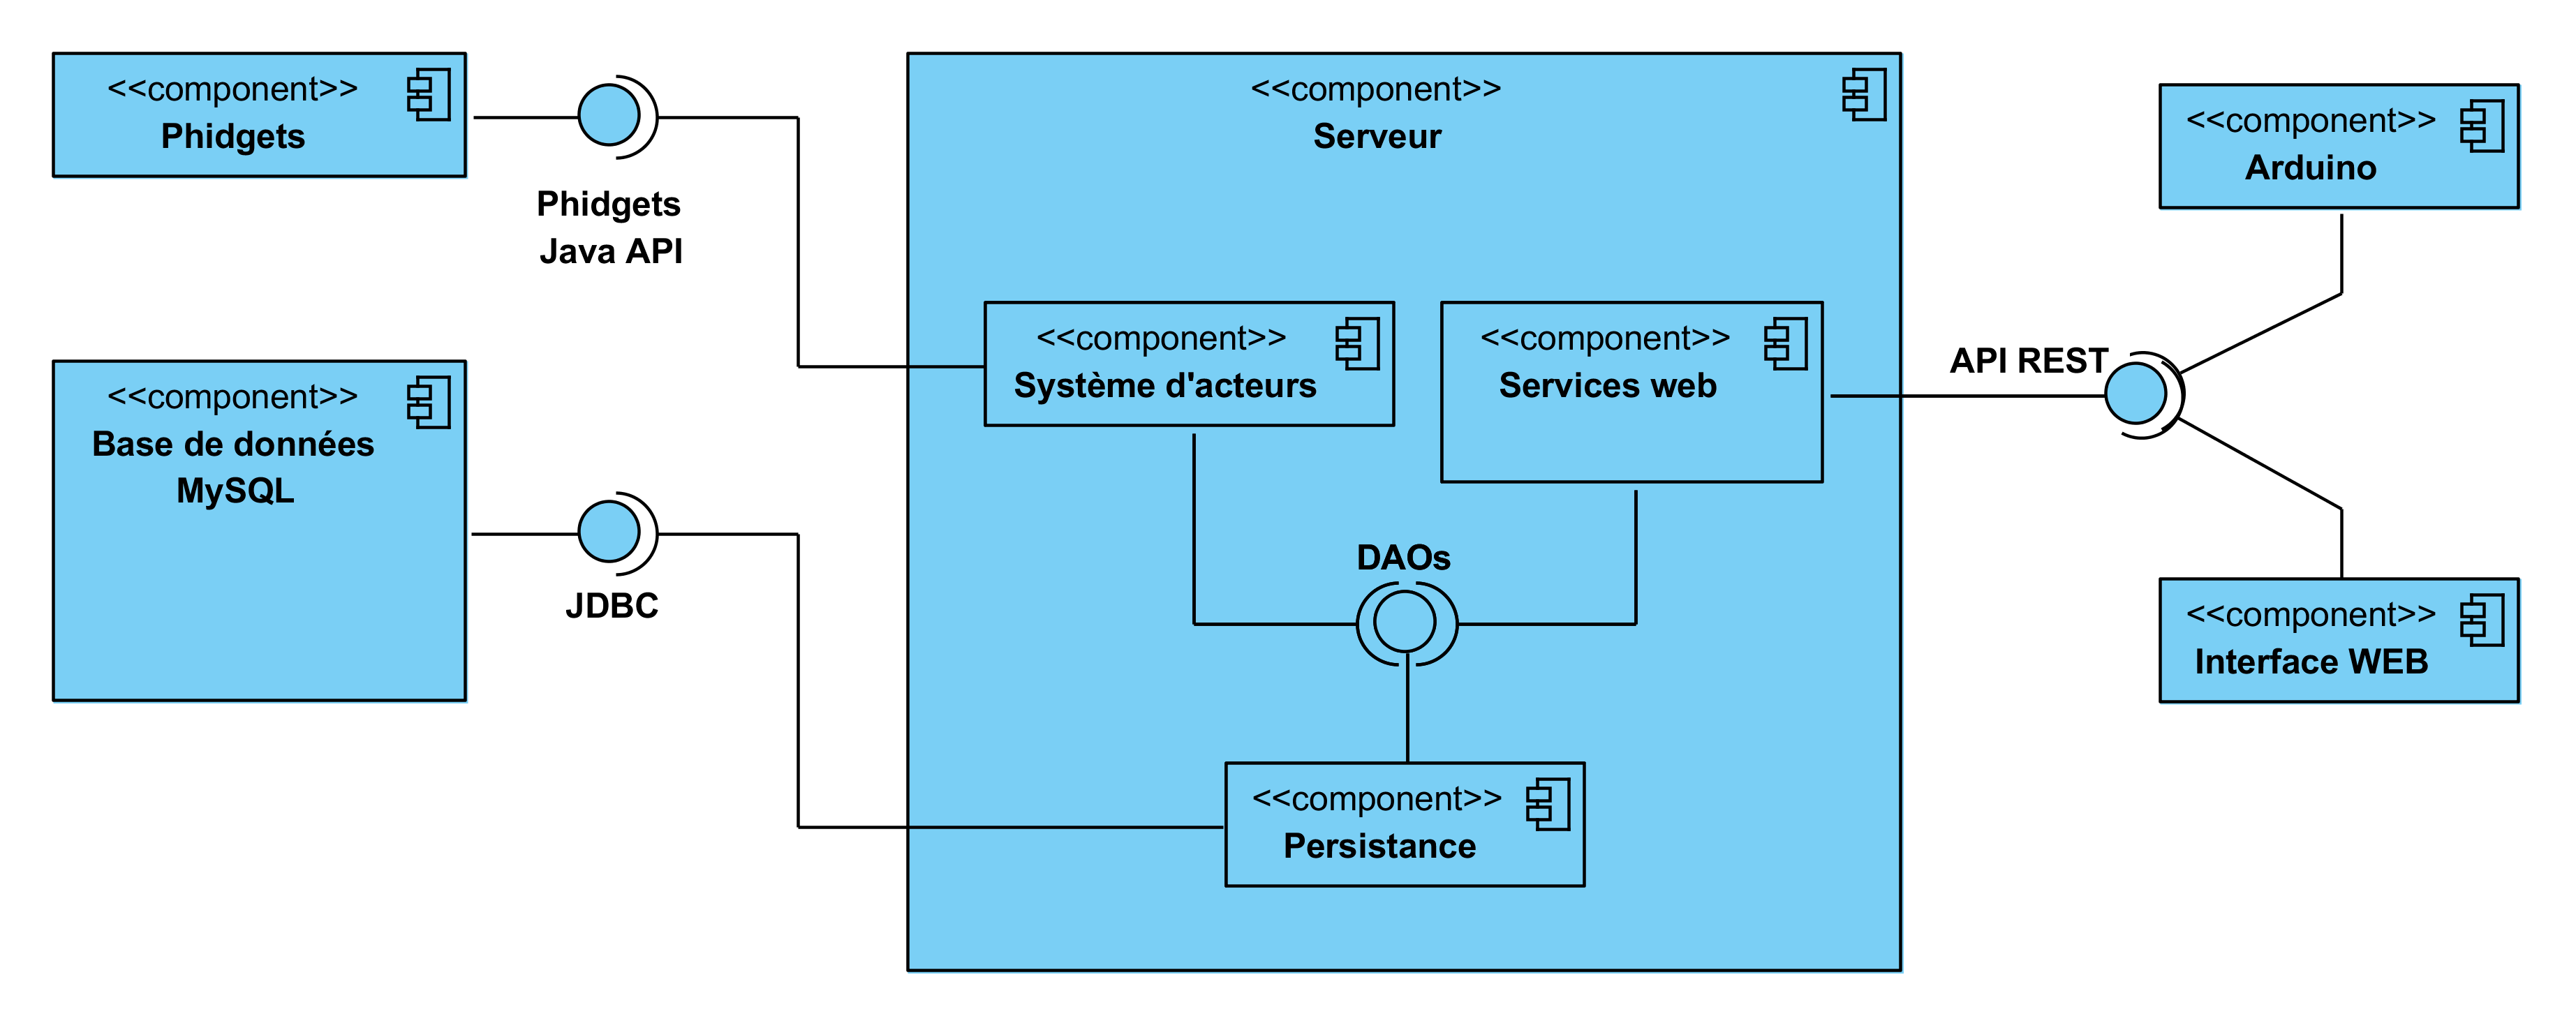
\includegraphics[width=\linewidth, height=\textheight,keepaspectratio]{img/diagramme-composants-archi-logi}}

        \caption{Diagramme de composants de l'architecture logicielle}
    \end{center}
\end{figure}
\subsection{Serveur}
Notre architecture logicielle côté serveur est basée sur une pile applicative reposant entièrement sur le langage Scala. Nous nous attarderons ici à décrire les 3 composants regroupés dans le serveur.\\

Néanmoins, quelques remarques préliminaires sont nécessaires :
\begin{itemize}
\item Pour faciliter le développement et surtout la gestion des dépendances, nous avons utilisé Maven. Lors de la phase de développement, le conteneur de servlets Jetty était utilisé. En phase de déploiement, nous avons choisi d’utiliser Tomcat 8 sur le Raspberry Pi (le WAR pouvant être facilement généré grâce à la commande : mvn:package).
\item Comme la librairie Java pour le Phidgets n’est pas disponible au travers d’un dépôt maven, il est nécessaire de l’importer localement sur la machine. Les instructions pour y parvenir sont disponibles en annexe.
\item Pour déployer le projet sur une machine de développement, il suffit d’exécuter la commande maven : mvn:jetty. En ce qui concerne le déploiement sur le Raspberry Pi, il est uniquement nécessaire de transférer le fichier WAR (préalablement généré) dans le dossier ‘webapps’ de Tomcat (l’auto-déploiement étant supposé activé).\\
\end{itemize}

Afin d’être complet, voici le diagramme de classes du composant “Serveur” :
\begin{figure}[H]
    \begin{center}
        \frame{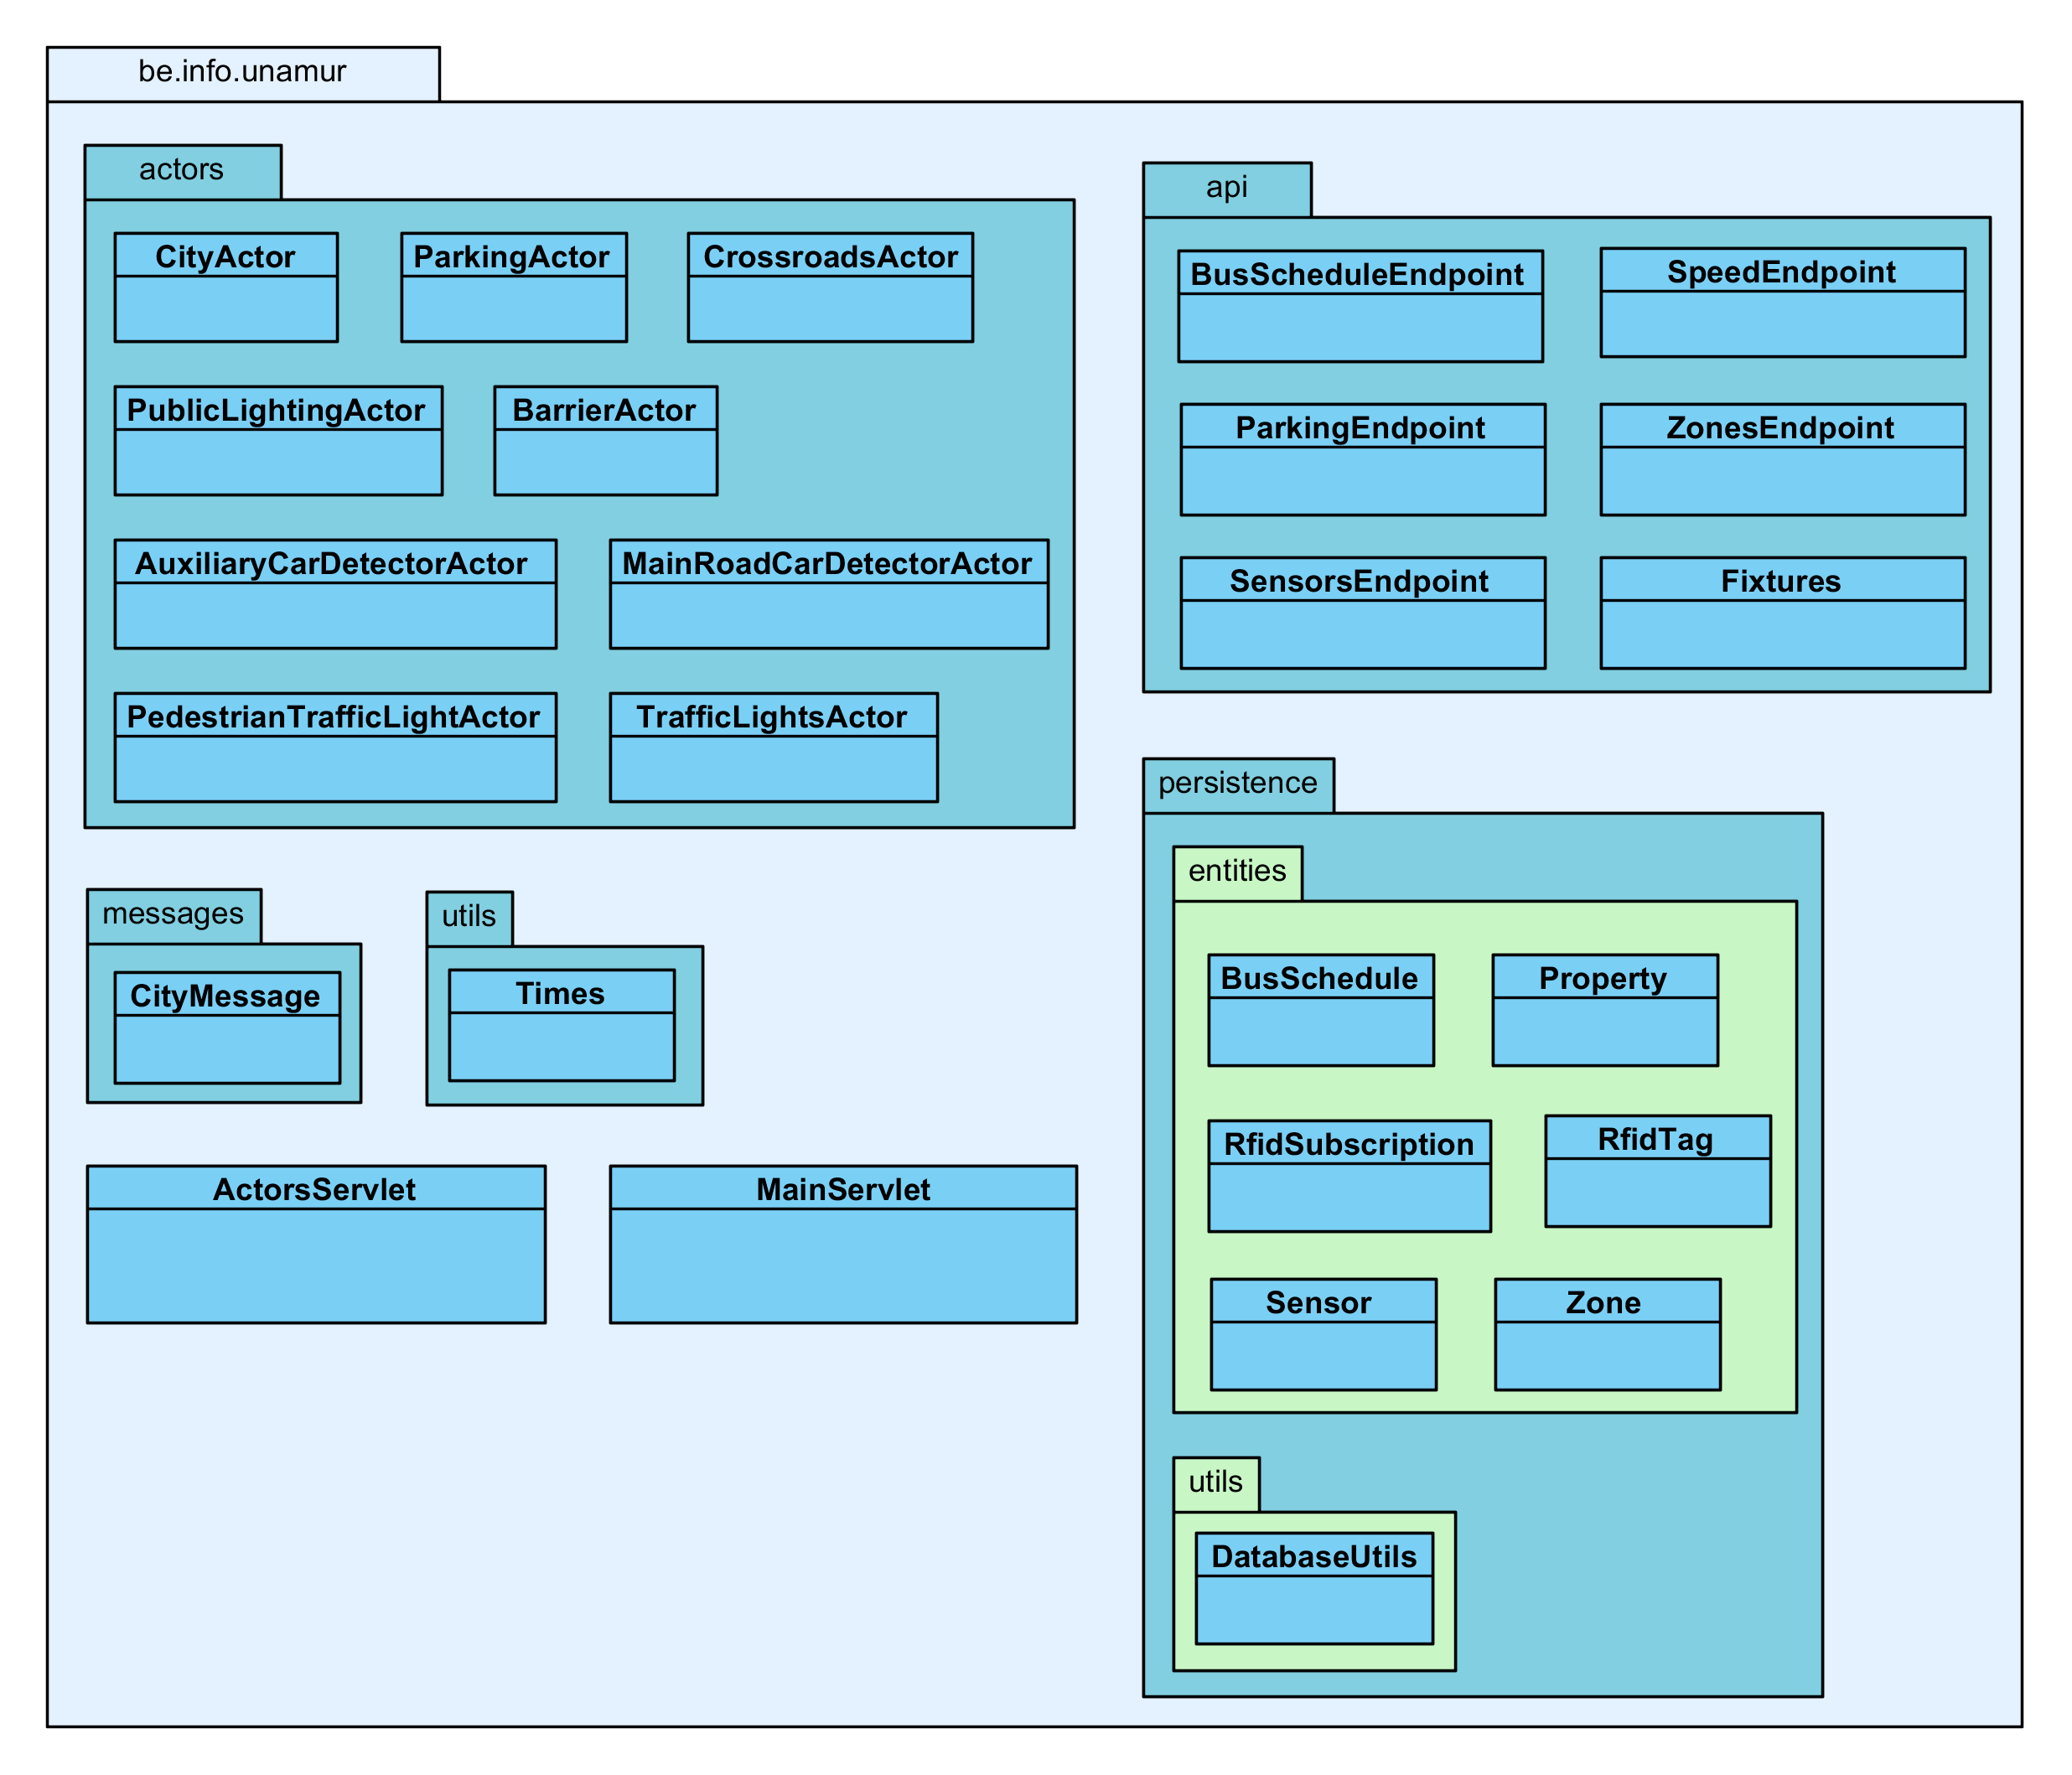
\includegraphics[width=\linewidth, height=\textheight,keepaspectratio]{img/diagramme-class-archi-logi}}

        \caption{Diagramme de class de l'architecture logicielle}
    \end{center}
\end{figure}

Intéressons-nous maintenant aux 3 composants principaux : le système d’acteurs, les services web et la « persistance » (c.-à-d. l’interaction avec la base de données).
\subsubsection{Système d'acteurs}\label{systeme-acteurs}
\subsubsection{Services web (API REST)}
\subsubsection{Persistence}